% ============================================================
\chapter{Learning on Manifolds}
\label{ch:manifolds}
% ============================================================

Graphs are discrete structures, but much data lives on \emph{continuous} non-Euclidean spaces: the surface of the Earth, the space of 3D rotations, the manifold of covariance matrices. Can one define neural networks directly on these \emph{differentiable manifolds}? The geometric approach to deep learning, systematised by Bronstein et al.\ in their 2021 ``blueprint,'' shows that this is possible---provided that Euclidean operations (convolution, translation) are replaced by their Riemannian analogues (parallel transport, exponential map). This chapter lays the necessary geometric foundations.

\section{Differential Geometry: Review}

\subsection{Differentiable Manifolds}

\begin{definition}[Differentiable manifold]
A \textbf{differentiable manifold} of dimension $d$ is a topological space
$\mathcal{M}$ that is locally homeomorphic to $\R^d$. More precisely, for
each point $p \in \mathcal{M}$, there exists an open neighborhood $U$ and a
homeomorphism (local chart) $\varphi: U \to \R^d$. The transition maps
$\varphi_\beta \circ \varphi_\alpha^{-1}$ are $C^\infty$.
\end{definition}

\begin{example}[Common manifolds]
\begin{enumerate}
    \item The \textbf{sphere} $S^2 = \{(x,y,z) \in \R^3 : x^2 + y^2 + z^2 = 1\}$
          --- dimension 2.
    \item The \textbf{torus} $T^2 = S^1 \times S^1$ --- dimension 2.
    \item The group $\mathrm{SO}(3)$ --- dimension 3.
    \item The space of symmetric positive definite matrices $\mathrm{Sym}^+(n)$.
\end{enumerate}
\end{example}

\subsection{Tangent Space and Riemannian Metric}

\begin{definition}[Tangent space]
The \textbf{tangent space} $T_p\mathcal{M}$ at a point $p \in \mathcal{M}$
is the vector space of tangent vectors to $\mathcal{M}$ at $p$. It has
dimension $d = \dim(\mathcal{M})$.
\end{definition}

\begin{definition}[Riemannian metric]
A \textbf{Riemannian metric} on $\mathcal{M}$ assigns to each
$p \in \mathcal{M}$ an inner product
$g_p: T_p\mathcal{M} \times T_p\mathcal{M} \to \R$ varying smoothly with $p$.
The pair $(\mathcal{M}, g)$ is a \textbf{Riemannian manifold}.
\end{definition}

\begin{keyformulas}[title=\textbf{Basic objects in Riemannian geometry}]
\begin{itemize}
    \item \textbf{Curve length} $\gamma: [0,1] \to \mathcal{M}$:
          $L(\gamma) = \int_0^1 \sqrt{g_{\gamma(t)}(\dot{\gamma}(t), \dot{\gamma}(t))}\, dt$
    \item \textbf{Geodesic distance}:
          $d(p, q) = \inf_\gamma L(\gamma)$ over curves connecting $p$ and $q$.
    \item \textbf{Exponential map}:
          $\exp_p: T_p\mathcal{M} \to \mathcal{M}$, sends $v$ to the point
          reached by the geodesic starting at $p$ in direction $v$.
    \item \textbf{Logarithmic map}:
          $\log_p: \mathcal{M} \to T_p\mathcal{M}$, (local) inverse of $\exp_p$.
\end{itemize}
\end{keyformulas}

\begin{figure}[htbp]
\centering
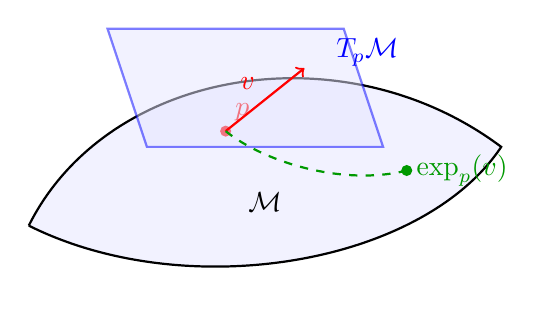
\begin{tikzpicture}
% Manifold (curved surface)
\draw[thick, fill=blue!5] (0,0) .. controls (1,2) and (4,2.5) .. (6,1)
    .. controls (5,-0.5) and (2,-1) .. (0,0);
\node at (3, 0.3) {$\mathcal{M}$};

% Point p
\fill[red] (2.5, 1.2) circle (2pt) node[above right] {$p$};

% Tangent plane
\draw[thick, blue, fill=blue!10, opacity=0.5]
    (1, 2.5) -- (4, 2.5) -- (4.5, 1) -- (1.5, 1) -- cycle;
\node[blue] at (4.3, 2.2) {$T_p\mathcal{M}$};

% Tangent vector
\draw[->, thick, red] (2.5, 1.2) -- (3.5, 2) node[midway, above left] {$v$};

% Geodesic
\draw[thick, green!60!black, dashed] (2.5, 1.2) .. controls (3, 0.8) and (4, 0.5) .. (4.8, 0.7);
\fill[green!60!black] (4.8, 0.7) circle (2pt) node[right] {$\exp_p(v)$};
\end{tikzpicture}
\caption{Tangent space, tangent vector, and exponential map.}
\end{figure}

\section{Differential Operators on Manifolds}

\begin{definition}[Laplace--Beltrami operator]
The \textbf{Laplace--Beltrami operator} generalizes the Laplacian to a
Riemannian manifold:
\[
    \Delta_{\mathcal{M}} f = \mathrm{div}(\mathrm{grad}\, f)
    = \frac{1}{\sqrt{\abs{g}}} \sum_{i,j} \partial_i\!\left(\sqrt{\abs{g}}\,
    g^{ij}\, \partial_j f\right)
\]
where $g^{ij}$ are the components of the inverse metric tensor and
$\abs{g} = \det(g_{ij})$.
\end{definition}

\begin{theorem}[Properties of $\Delta_{\mathcal{M}}$]
\begin{enumerate}
    \item $\Delta_{\mathcal{M}}$ is \textbf{self-adjoint} and \textbf{negative semi-definite}
          (with the convention $\Delta f = -\mathrm{div}(\nabla f)$ the sign is reversed).
    \item It is \textbf{intrinsic}: independent of the coordinate system.
    \item It generalizes the graph Laplacian: on a graph, $\mathbf{L}$ is a
          discretization of $-\Delta_{\mathcal{M}}$.
    \item It admits a spectral decomposition:
          $\Delta_{\mathcal{M}} \phi_k = -\lambda_k \phi_k$ with
          $0 = \lambda_0 \leq \lambda_1 \leq \cdots$
\end{enumerate}
\end{theorem}

\begin{proposition}[Heat equation on $\mathcal{M}$]
The heat equation on a manifold reads:
\[
    \frac{\partial u}{\partial t} = \Delta_{\mathcal{M}} u
\]
Its solution is $u(p, t) = \int_{\mathcal{M}} K_t(p, q)\, u_0(q)\, dq$ where
$K_t(p,q) = \sum_k e^{-\lambda_k t} \phi_k(p) \phi_k(q)$ is the
\textbf{heat kernel}.
\end{proposition}

\section{Convolutions on Manifolds}

\subsection{Challenges}

On a manifold, classical convolution poses several challenges:
\begin{itemize}
    \item No \textbf{translation group structure} (except for $\R^n$ and the torus).
    \item No \textbf{global coordinate system}.
    \item \textbf{Parallel transport} is needed to compare vectors at different points.
\end{itemize}

\subsection{Spectral Approach: MoNet and Variants}

\begin{definition}[MoNet --- Monti et al., 2017]
MoNet (\textit{Mixture Model Networks}) defines parametric filters in local
pseudo-polar coordinates:
\[
    \mathbf{h}_v^{(\ell+1)} = \sum_{j=1}^{J} \mathbf{W}_j^{(\ell)}
    \sum_{u \in \mathcal{N}(v)} w_j(\mathbf{c}(v, u))\, \mathbf{h}_u^{(\ell)}
\]
where $\mathbf{c}(v, u) = (\rho_{vu}, \theta_{vu})$ are pseudo-polar
coordinates of $u$ in the local frame of $v$, and
$w_j(\mathbf{c}) = \exp\!\left(-\frac{1}{2}(\mathbf{c} - \boldsymbol{\mu}_j)^\top
\boldsymbol{\Sigma}_j^{-1}(\mathbf{c} - \boldsymbol{\mu}_j)\right)$
are learned Gaussian kernels.
\end{definition}

\subsection{Convolution via Spectral Descriptors}

\begin{definition}[Diffusion kernel]
The \textbf{diffusion kernel} of a manifold is defined by:
\[
    K_t(p, q) = \sum_{k=0}^{\infty} e^{-\lambda_k t}\, \phi_k(p)\, \phi_k(q)
\]
It defines an inner product in a reproducing kernel Hilbert space (RKHS) and
provides intrinsic shape descriptors.
\end{definition}

\begin{definition}[HKS --- Heat Kernel Signature]
The \textbf{Heat Kernel Signature} is an intrinsic descriptor of local geometry:
\[
    \mathrm{HKS}(p, t) = K_t(p, p) = \sum_{k=0}^{\infty} e^{-\lambda_k t}\, \phi_k(p)^2
\]
It encodes multi-scale information: small $t$ captures local geometry, large
$t$ captures global geometry.
\end{definition}

\begin{codeblock}[title=\textbf{Computing HKS on a mesh}]
\begin{minted}{python}
import torch
import numpy as np

def compute_hks(eigenvalues, eigenvectors, time_scales):
    """Compute Heat Kernel Signature.

    Args:
        eigenvalues: (K,) Laplacian eigenvalues
        eigenvectors: (N, K) eigenvectors
        time_scales: (T,) time scales
    Returns:
        hks: (N, T) HKS descriptors
    """
    exp_vals = torch.exp(
        -eigenvalues.unsqueeze(1) * time_scales.unsqueeze(0)
    )
    phi_sq = eigenvectors ** 2
    hks = phi_sq @ exp_vals  # (N, T)
    return hks

eigenvalues = torch.linspace(0, 10, 100)
eigenvectors = torch.randn(500, 100)
eigenvectors, _ = torch.linalg.qr(eigenvectors)
time_scales = torch.logspace(-2, 2, 16)

hks = compute_hks(eigenvalues, eigenvectors[:, :100], time_scales)
print(f"HKS descriptors: {hks.shape}")  # (500, 16)
\end{minted}
\end{codeblock}

\section{Convolution via Parallel Transport}

\begin{definition}[Parallel transport]
\textbf{Parallel transport} along a curve $\gamma: [0,1] \to \mathcal{M}$
is a linear map $\Gamma_\gamma: T_{\gamma(0)}\mathcal{M} \to
T_{\gamma(1)}\mathcal{M}$ that transports a tangent vector along $\gamma$
while preserving the inner product and satisfying:
\[
    \nabla_{\dot{\gamma}} V = 0
\]
where $\nabla$ is the Levi-Civita connection.
\end{definition}

\begin{definition}[Gauge Equivariant CNN --- de Haan et al., 2021]
A \textbf{Gauge Equivariant CNN} defines convolutions on a manifold using
\textbf{local frames} (gauges) and parallel transport:
\[
    [f * \psi](p) = \int_{\mathcal{M}} f(\Gamma_{q \to p}\, \cdot)\,
    \psi(\exp_p^{-1}(q))\, dq
\]
The network is equivariant to gauge changes: the choice of local frame does
not affect the output.
\end{definition}

\section{Learning on Specific Manifolds}

\subsection{Convolutions on the Sphere}

\begin{definition}[Spherical CNN --- Cohen et al., 2018]
\textbf{Spherical CNNs} define convolutions on $S^2$ using spherical
harmonics as a spectral basis:
\[
    [f * \psi](\hat{\mathbf{r}}) = \sum_{\ell=0}^{L} \sum_{m=-\ell}^{\ell}
    \hat{f}_\ell^m\, \hat{\psi}_\ell\, Y_\ell^m(\hat{\mathbf{r}})
\]
where $\hat{f}_\ell^m$ and $\hat{\psi}_\ell$ are coefficients in the spherical
harmonics basis. For a \textbf{zonal} filter (rotationally symmetric),
$\hat{\psi}_\ell$ depends only on $\ell$.
\end{definition}

\begin{theorem}[$\mathrm{SO}(3)$ equivariance]
Spherical convolution is rotation-equivariant: if $R \in \mathrm{SO}(3)$ and
$L_R f(\hat{\mathbf{r}}) = f(R^{-1}\hat{\mathbf{r}})$, then:
\[
    L_R(f * \psi) = (L_R f) * \psi
\]
\end{theorem}

\subsection{Learning on Lie Groups}

\begin{definition}[LieConv --- Finzi et al., 2020]
LieConv defines convolutions directly on Lie groups using a \textbf{continuous
kernel} parameterized in the Lie algebra:
\[
    [f * \psi](g) = \int_G f(h)\, \psi(\log(h^{-1}g))\, d\mu(h)
\]
In practice, the integral is approximated by Monte Carlo on a sampled
neighborhood.
\end{definition}

\section{Applications: 3D Shape Analysis}

\begin{definition}[Shape correspondence]
The \textbf{shape correspondence} problem seeks a map
$T: \mathcal{M}_1 \to \mathcal{M}_2$ between two surfaces that preserves
geometric structure. Spectral methods use \textbf{functional maps}:
\[
    \mathbf{C} = \boldsymbol{\Phi}_2^\dagger\, T_f\, \boldsymbol{\Phi}_1
\]
where $\boldsymbol{\Phi}_i$ are the truncated eigenfunction matrices and
$T_f$ is the functional correspondence operator.
\end{definition}

\begin{codeblock}[title=\textbf{Functional maps for shape correspondence}]
\begin{minted}{python}
import torch

def functional_map(phi_1, phi_2, descriptors_1, descriptors_2, k=30):
    """Compute a functional map.

    Args:
        phi_1, phi_2: (N, k) truncated eigenfunctions
        descriptors_1, descriptors_2: (N, d) descriptors (HKS, etc.)
        k: number of eigenfunctions
    Returns:
        C: (k, k) functional map matrix
    """
    A1 = phi_1[:, :k].T @ descriptors_1  # (k, d)
    A2 = phi_2[:, :k].T @ descriptors_2  # (k, d)
    C, _ = torch.linalg.lstsq(A1.T, A2.T)
    C = C.T  # (k, k)
    return C

N = 1000
k = 30
phi_1 = torch.randn(N, k)
phi_2 = torch.randn(N, k)
desc_1 = torch.randn(N, 16)
desc_2 = torch.randn(N, 16)
C = functional_map(phi_1, phi_2, desc_1, desc_2, k=k)
print(f"Functional map: {C.shape}")  # (30, 30)
\end{minted}
\end{codeblock}

\section{Optimization on Manifolds}

\begin{definition}[Riemannian gradient]
The \textbf{Riemannian gradient} of a function $f: \mathcal{M} \to \R$ at $p$
is the unique vector $\mathrm{grad}\, f(p) \in T_p\mathcal{M}$ such that:
\[
    g_p(\mathrm{grad}\, f(p), v) = df_p(v), \quad \forall v \in T_p\mathcal{M}
\]
\end{definition}

\begin{algorithme}[title=\textbf{Riemannian gradient descent}]
\begin{enumerate}
    \item Compute the Euclidean gradient $\nabla f(\mathbf{x})$.
    \item Project onto the tangent space: $\xi = \mathrm{Proj}_{T_\mathbf{x}\mathcal{M}}(\nabla f)$.
    \item Perform a retraction step: $\mathbf{x}' = \mathrm{Retr}_\mathbf{x}(-\eta\, \xi)$.
\end{enumerate}
For $\mathrm{SO}(n)$, the retraction is $\mathrm{Retr}_Q(\xi) = \mathrm{qr}(Q + \xi)$.
\end{algorithme}

\begin{codeblock}[title=\textbf{Optimization on the sphere with geoopt}]
\begin{minted}{python}
import torch
import geoopt

# Variable on the sphere S^{n-1}
sphere = geoopt.Sphere()
x = sphere.random(torch.Size([10]), dtype=torch.float)
x = geoopt.ManifoldParameter(x, manifold=sphere)

# Objective: minimize distance to a target point
target = sphere.random(torch.Size([10]), dtype=torch.float)
optimizer = geoopt.optim.RiemannianAdam([x], lr=0.01)

for step in range(100):
    optimizer.zero_grad()
    loss = (x - target).norm() ** 2
    loss.backward()
    optimizer.step()

print(f"Final distance: {(x - target).norm():.6f}")
print(f"On sphere: {x.norm():.6f}")  # should be ~1
\end{minted}
\end{codeblock}

\section*{Exercises}

\begin{exercise}[Laplace--Beltrami on the sphere]
\begin{enumerate}
    \item Show that spherical harmonics $Y_\ell^m$ are eigenfunctions of
          $\Delta_{S^2}$ with eigenvalues $\lambda_\ell = \ell(\ell+1)$.
    \item Compute the first spherical harmonics and visualize them.
\end{enumerate}
\end{exercise}

\begin{exercise}[Heat kernel]
\begin{enumerate}
    \item Analytically compute the heat kernel on the circle $S^1$.
    \item Implement numerical computation of the heat kernel on a triangular mesh.
    \item Visualize heat diffusion at different scales $t$.
\end{enumerate}
\end{exercise}

\begin{exercise}[Parallel transport]
\begin{enumerate}
    \item Compute parallel transport along a meridian of the sphere.
    \item Show that parallel transport around a spherical triangle induces a
          rotation by an angle equal to the spherical excess.
    \item Implement discrete parallel transport on a mesh.
\end{enumerate}
\end{exercise}

\begin{exercise}[Shape correspondence]
Implement a shape correspondence pipeline using:
\begin{enumerate}
    \item HKS descriptors as node features.
    \item A GNN to learn equivariant descriptors.
    \item Functional maps for correspondence.
\end{enumerate}
\end{exercise}
